\documentclass{beamer}

\mode<presentation>
{
  \usetheme{default}      
  \usecolortheme{default}
  \usefonttheme{default}  
  \setbeamertemplate{navigation symbols}{}
  \setbeamertemplate{caption}[numbered]
} 

\usepackage[english]{babel}
\usepackage[utf8x]{inputenc}

\title[presentationTemplate]{Computation Tree Logic}
\author{Luis Tertulino \& Ronaldo Silveira}
\date{\today}

\usepackage{amsthm, amssymb, amsfonts, amsmath}
\usepackage{graphicx}
\usepackage{tikz}
\usetikzlibrary{calc,shapes}
\usepackage{enumitem}
\usepackage{mathtools}
\usepackage{mathrsfs}
\usepackage{tikz-cd}
%usepackage{lstlist}

\newcommand{\C}{\mathbb{C}}
\newcommand{\R}{\mathbb{R}}
\newcommand{\Q}{\mathbb{Q}}
\newcommand{\Z}{\mathbb{Z}}
\newcommand{\N}{\mathbb{N}}
\newcommand{\p}{\mathbb{P}}
\newcommand{\E}{\mathbb{E}}

\AtBeginSubsection[]
{
  \begin{frame}
    \tableofcontents[currentsection,currentsubsection]
  \end{frame}
}


\begin{document}

\begin{frame}
	\titlepage
\end{frame}

\begin{frame}
\tableofcontents
\end{frame}

\section{In previous chapters...}
\subsection{Temporal Logic}


\section{In previous chapters...}
\subsection{Temporal Logic}
\begin{frame}{Previously on Temporal Logic Week...}
  \framesubtitle{Temporal Logic}
  \begin{itemize}
	\item
  \end{itemize}

\end{frame}
\section{Introduction}
\begin{frame}{Motivation}
	\begin{itemize}
		\item 
		{
			Needing of uncertainty;
			\pause
		} 
		\item 
		{
			Different paths of the future;
		}
	\end{itemize}
\end{frame}
\begin{frame}{Intuition}
	In Computation Tree Logic (CTL) the model of time is a tree-like structure. This way, we cannot use Linear Temporal Logic (LTL) to express the existence of a certain path of time in which some event occurs.
\end{frame}

\begin{frame}{History}
    CTL was defined by:
    
    \begin{columns}[c]
        \begin{column}{.3\textwidth}
            \begin{figure}
                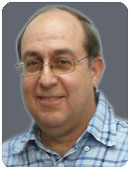
\includegraphics[scale=2]{images/benari.jpg}
                \caption{Mordechai Ben-Ari}
            \end{figure}
        \end{column}
        \begin{column}{.3\textwidth}
            \begin{figure}
                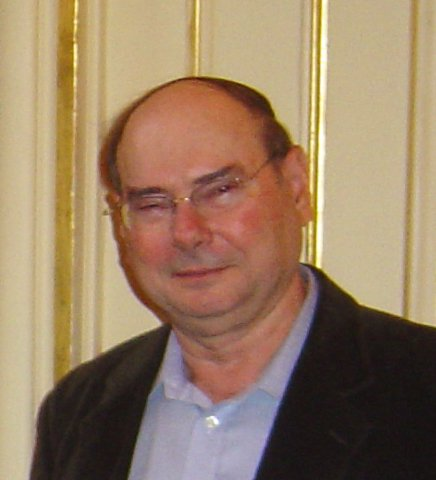
\includegraphics[scale=0.17]{images/Amir_Pnueli.jpg}
                \caption{Amir Pnueli}
            \end{figure}
        \end{column}
        \begin{column}{.3\textwidth}
            \begin{figure}
                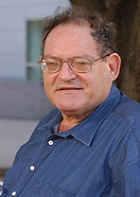
\includegraphics[scale=0.5]{images/manna.jpg}
                \caption{Zohar Manna}
            \end{figure}
        \end{column}
        
    \end{columns}
    
\end{frame}


\begin{frame}{History}
    And, at the same time by:
    
    \begin{columns}[c]
        \begin{column}{.3\textwidth}
            \begin{figure}
                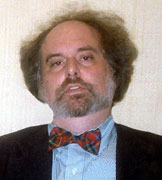
\includegraphics[scale=0.5]{images/E_Allen_Emerson.jpg}
                \caption{Ernest Allen Emerson}
            \end{figure}
        \end{column}
        \begin{column}{.3\textwidth}
            \begin{figure}
                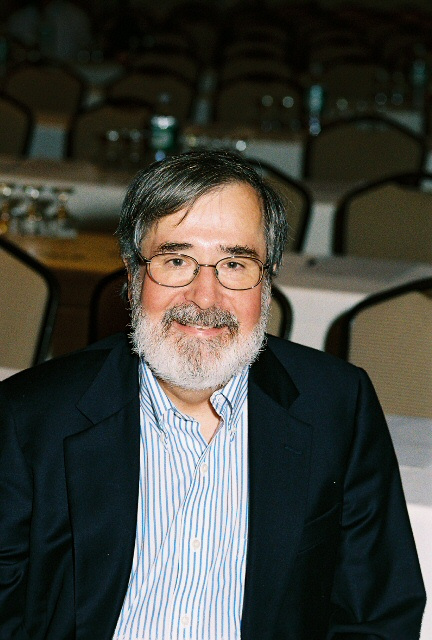
\includegraphics[scale=0.17]{images/Edmund_Clarke.jpg}
                \caption{Edmund Clarke}
            \end{figure}
        \end{column}
    \end{columns}
    
\end{frame}
\section{How to communicate}
\subsection{Syntax of CTL}
\begin{frame}{Syntax}
	\framesubtitle{Definition}
	The syntax of CTL consists on the syntax of temporal logic plus some path operators. The class of formulas can be defined in Backus-Naur form. If $\phi$ is a formula: \pause
	$$\phi ::= \bot \; | \; \top \; | \; p \; | \; \neg \phi \; | \; \phi \land \phi \; | \; \phi \lor \phi \; | \; \phi \to \phi \; | \; \A\X \phi \; | \; \E\X \phi \; | $$
	$$\A\F \phi \; | \; \E\F \phi \; | \; \A\G \phi \; | \; \E\G \phi \; | \; \A[\phi \U \phi] \; | \; \E[\phi \U \phi]$$\pause
	
	With $p$ as a literal (atomic formula), \A\X, \E\X, \A\F, \E\F, \A\G \, e \E\G \, unary operators.
	
\end{frame}

\begin{frame}{Syntax}
	\framesubtitle{Intuition}
	The propositional operators: $\neg, \lor, \land, \to$ have the same meaning of in the propositional logic.\pause
	
	The temporal operators can be read (if $\varphi$ is a formula) as follows: \pause
	\begin{itemize}
		\item 
		{
			$\A \varphi$: $\varphi$ is true in all possible paths;
			\pause
		}
		\item 
		{
			$\E \varphi$: $\varphi$ exists a path in which $\phi$ is true;
			\pause
		}
	\end{itemize}
	
	The path-specific operators can be read, considering $\varphi$ and $\psi$ formulas, as: \pause
	\begin{itemize}
		\item 
		{
			$\X \varphi:$ $\varphi$ is  true until next state;
			\pause
		}
		\item 
		{
			$\F \varphi:$ There is some state in the future where $\varphi$ is true;
			\pause
		}
		\item
		{
			$\G \varphi: $ Globally (in all future states) $\varphi$ is true;
			\pause
		}
		\item
		{
			$\varphi \U \psi$: $\varphi$ is true at least until $\psi$ becomes true;	
		}
	\end{itemize}
	
\end{frame}

\begin{frame}{Syntax}
	\framesubtitle{Notes}
	\begin{itemize}
		\item 
		{
			Notice that, in CTL, the combination of path specific operators and temporal operators are atomic, i.e., \A\F \; is a operator that can be read as ``In all paths in the future there is some state where...''
			\pause
		}
		
		\item 
		{
			Notice as well that the binary operators $\A[\varphi\U\psi]$ and $\E[\varphi\U\psi]$ can be represented as \A\U
			\pause
		}
		
		\item 
		{
			We assume that, similarly to the $\neg$ operator, the ``new'' unary operators ($\A\X, \E\X, \A\F, \E\F, \A\G $, and $ \E\G $) have the first precedence. Next comes the $\land$ and $\lor$ operators. And at last the $\to$, $\A\U$ and $\E\U$
			\pause
		}
	\end{itemize}
	
\end{frame}

\begin{frame}{Examples}
	\begin{itemize}
		\item
		{
			Examples of well-formed formulas:
			\begin{itemize}
				\item $\A\G (p \lor \E\F q)$ \pause
				\item $\A\X (q \to \E[(p\lor q) \U r])$ \pause
				\item $\E\F\E\G p \to \A\F r$ Note that this is binded as $(\E\F\E\G p) \to \A\F r$, not as $\E\F\E\G (p \to \A\F r)$
			\end{itemize}
			\pause
		}
		\item
		{
			Example of formulas that are not well-formed:
			\begin{itemize}
				\item $\A\neg\G \neg p$ \pause
				\item $F[p\U s]$ \pause
				\item $A[p\U s \land q \U s]$
			\end{itemize}
		}
	\end{itemize}
\end{frame}


\subsection{Semantics of CTL}
\begin{frame}{Semantics}
	\framesubtitle{Definition of model}
	Different from usual logics, CTL formulas are interpreted by a transition system. Given an set of atoms:\pause
	\begin{definition}[1]
		A \alert{transition system} $\M$ is a triple $\M = (S, \to, L)$ in which $S$ is a set of states, $\to$ is a binary relation over $S$ ($\to \subseteq S\times S$) and $L: S \to \mathcal{P}(Atoms)$ is a labelling function.
	\end{definition}\pause
	\begin{definition}[2]
		A \alert{model} is a duple $\M,s$ in which $\M$ is a transition system and $s$ is a state.
	\end{definition}\pause
	
	{\bf Notation:} we will use $\M,s\vDash \varphi$ to denote that the model $\M,s$ satisfies the formula $\varphi$
\end{frame}


\begin{frame}{Semantics}
	\framesubtitle{Satisfaction}
	Take an arbitrary model $\M$. Let $s, s_1, s_2, s_3$ be states in $S$. Let $\varphi, \varphi_1, \varphi_2$ be well-formed formulas of CTL. And let $p$ be an atom. The satisfaction of CTL formulas can be defined as follows:
	\begin{itemize}
		\item $\M,s \vDash \top$ and $\M,s \not\vDash \bot$ for all $s \in S$ \pause
		\item $\M,s \vDash p$ iff $p \in L(S)$ \pause
		\item $\M,s \vDash \neg\varphi$ iff $\M,s \not\vDash \varphi$ \pause
		\item $\M,s \vDash \varphi_1 \land \varphi_2$ iff $\M,s \vDash \varphi_1$ AND $\M,s \vDash \varphi_2$ \pause
		\item $\M,s \vDash \varphi_1 \lor \varphi_2$ iff $\M,s \vDash \varphi_1$ OR $\M,s \vDash \varphi_2$ \pause
		\item $\M,s \vDash \varphi_1 \to \varphi_2$ iff $\M,s \not\vDash \varphi_1$ OR $\M,s \vDash \varphi_2$
	\end{itemize}
\end{frame}

\begin{frame}{Semantics}
	\framesubtitle{Satisfaction}
	Take an arbitrary model $\M$. Let $s, s_1, s_2, s_3$ be states in $S$. Let $\varphi, \varphi_1, \varphi_2$ be well-formed formulas of CTL. And let $p$ be an atom. The satisfaction of CTL formulas can be defined as follows:
	\begin{itemize}
		\item $\M,s \vDash \A\X \varphi$ iff for all $s_1$ that $s \to s_1$ and $\M,s_1 \vDash \varphi$. Thus, $\A\X$ says: ``in every next state...''\pause
		\item $\M,s \vDash \E\X \varphi$ iff exists $s_1$ that $s \to s_1$ and $M,s_1 \vDash \varphi$. Thus, $\E\X$ says: ``in some next state...''\pause
		\item $M,s, \vDash \A\G \varphi$ iff for all paths $s_1 \to s_2 \to s_3 \to ...$ in which $s = s_1$, for all $s_i$, $M, s_i \vDash \varphi$. Thus, $\A\G$ says: ``In all possible paths from now on in all next states...''\pause
		\item $M,s, \vDash \A\G \varphi$ iff exists some path $s_1 \to s_2 \to s_3 \to ...$ in which $s = s_1$, for all $s_i$, $M, s_i \vDash \varphi$ Thus, $\E\G$ says: ``Exists a path from now on in all next states...''\pause
	\end{itemize}
\end{frame}

\begin{frame}{Semantics}
	\framesubtitle{Satisfaction}
	Take an arbitrary model $\M$. Let $s, s_1, s_2, s_3$ be states in $S$. Let $\varphi, \varphi_1, \varphi_2$ be well-formed formulas of CTL. And let $p$ be an atom. The satisfaction of CTL formulas can be defined as follows:
	\begin{itemize}
		\item $M,s, \vDash \A\F \varphi$ iff for all paths $s_1 \to s_2 \to s_3 \to ...$ in which $s = s_1$, exists $s_i$, $M, s_i \vDash \varphi$. Thus, $\A\F$ says: ``In all possible paths from now on, in some next state...''\pause
		\item $M,s, \vDash \E\F \varphi$ iff exists some path $s_1 \to s_2 \to s_3 \to ...$ in which $s = s_1$, that exists $s_i$, $M, s_i \vDash \varphi$. Thus, $\E\F$ says: ``In some path from now on, in some next state...''\pause
		\item $M,s, \vDash \A[\varphi_1 \U \varphi_2]$ iff for all paths $s_1 \to s_2 \to s_3 \to ...$ in which $s = s_1$, this path satisfies $\varphi_1 \U \varphi_2$, i.e., exists $s_i$ in the path such that $\M, s_i \vDash \varphi_2$ and, for all $j < i$, $M, s_j \vDash \varphi_1$. Thus, $\A\U$ says: ``For all paths from now on, until some state...''\pause
		\item $M,s, \vDash \E[\varphi_1 \U \varphi_2]$ iff exists some path $s_1 \to s_2 \to s_3 \to ...$ in which $s = s_1$, this path satisfies $\varphi_1 \U \varphi_2$. Thus, $\E\U$ says: ``In some path from now on, until some state...''
	\end{itemize}
\end{frame}
\section{Some examples of what we can say}
\begin{frame}{Examples}
	\begin{itemize}
		\item 
		{
			``It's possible to get to a state where something has started but it's not ready'': $\E\F(started \land \neg ready)$ 
			\pause
		}
		\item
		{
			``A certain process is enabled infinitely often on every computation path'': $\A\G(\A\F enabled)$	
			\pause
		}
		\item
		{
			``An upwards travelling lift at the second floor does not change its direction when it has passengers wishing to go to the fifth floor'': $\A\G(floor2 \land directionup \land button5 \to \A[directionup \U floor5])$
		}
	\end{itemize}
\end{frame}
\section{More about semantics}
\subsection{Equivalences}

\begin{frame}{Equivalences}
	\begin{definition}
		Two CTL formulas $\varphi$ and $\psi$ are said to be \alert{semantically	equivalent} if any state in any model which satisfies one of them also satisfies the other; 
	\end{definition}\pause
	\textbf{Notation:} we denote the semantic equivalence of $\varphi$ and $\psi$ by $\varphi \equiv \psi$
\end{frame}

\begin{frame}{Example of equivalences}
    Let $\varphi$ be an arbitrary CTL formula.
        
    \begin{itemize}
        \item
        {
            $\neg \A\F \varphi \equiv \E\G \neg \varphi $    
            \pause
        }
        \item
        {
            $\neg \E\F \varphi \equiv \A\G \neg \varphi$    
            \pause    
        }
        \item
        {
            $\neg \A\X \varphi \equiv \E\X \neg \varphi$    
            \pause
        }
        \item
        {
            $\A\F\varphi \equiv \A[\top \U\varphi]$    
            \pause
        }
        \item
        {
            $\E\F \varphi \equiv \E[\top \U\varphi]$
        }
    \end{itemize}
\end{frame}

\begin{frame}{Minimum set of CTL connectives}
    Because of the equivalences shown and the ones in propositional logic, we can have some minimum sets of conectives for the CTL syntax. One of them is defined in Backus-Naur formalism below:
    $$\phi ::=  \bot \; | \; p \; | \; \neg \phi \; | \; \phi \land \phi \; | \; \E\X \phi \; | \;  \A\F\phi \; | \; \E[\phi\U\phi]$$
\end{frame}
\section{Improving our language}
\begin{frame}{Needing some more?}
    Even if CTL allow explicit quantification over paths, it cannot allow some expressions to be formed.
\end{frame}
\section{Model checking algorithms}

\begin{frame}{The CTL model-checking algorithm}
	\begin{itemize}
		\item
		{
			Given a property of a program expressed in a temporal logic, the model checker checks if the states of the program satisfy the formula.
			\pause
		}
		\item
		{
			Obviously, we use CTL formulas.
			\pause
		}
		\item
		{
			There are two different ways of working with model checking:\\
			\pause
			Given a model, a state and a formula, tells if the model and the state satisfies the formula;\\
			\pause
			Given a model and a formula, returns the set of states that satisfies the formula.
		}
	\end{itemize}
\end{frame}

\begin{frame}{The CTL model-checking algorithm}
	\framesubtitle{The labelling algorithm}
	We present an algorithm that, given a model and a CTL formula, outputs the set of states of the model that satisfy the formula. 
\end{frame}

\begin{frame}{The CTL model-checking algorithm}
	\framesubtitle{The labelling algorithm}
	The algorithm deals explicitly only with some of the CTL connectives; for the others, it transforms them to their equivalent form in terms of the minimal set of connectives previously defined: $\{\bot, \neg, \land, \A\F, \E\U, \E\X \}$ 
\end{frame}

\begin{frame}{The CTL model-checking algorithm}
	\framesubtitle{The labelling algorithm}
	Here is the algorithm:\\
	\pause
	{\bf INPUT}: a CTL model $\M = (S, \to, L)$ and a CTL formula $\phi$.\\
	{\bf OUTPUT}: the set of states of $\M$ which satisfies $\phi$.\\
	\pause
	\begin{itemize}
		\item
		{
			First, rewrite $\phi$ in terms of $\bot, \neg, \land, \A\F, \E\U$ and $\E\X$.
			\pause
		}
		\item
		{
			Next, label the states of $\M$ with the subformulas of $\phi$ that are satisfied there, starting with the smallest subformulas and working outwards towards $\phi$.
		}
	\end{itemize}
\end{frame}

\begin{frame}{The CTL model-checking algorithm}
	\framesubtitle{The labelling algorithm}
	Suppose $\psi$ is a subformula of $\phi$ and states satisfying all the immediate subformulas of $\psi$ have already been labeled. We determine by a case analysis which states to label with $\psi$. If $\psi$ is
	
	\begin{itemize}
		\item
		{
			$\bot$: then no states are labeled with $\bot$.
			\pause
		}
		\item
		{
			$p$: then label $s$ with $p$ if $p \in L(s)$.
			\pause
		}
		\item
		{
			$\psi_{1} \land \psi_{2}$: label $s$ with $\psi_{1}$ ? $\psi_{2}$ if $s$ is already labeled both with $\psi_{1}$ and with $\psi_{2}$.
			\pause
		}
		\item
		{
			$\neg \psi_{1}$: label $s$ with $\neg \psi_{1}$ if $s$ is not already labeled with $\psi_{1}$.
			\pause
		}
		\item
		{
			$\A\F \psi_{1}$:
			\begin{itemize}
				\item If any state $s$ is labeled with $\psi_{1}$, label it with $\A\F \psi_{1}$.
				\item Repeat: label any state with $\A\F \psi_{1}$ if all successor states are labeled with $\A\F \psi_{1}$, until there is no change.
			\end{itemize} 
		}
	\end{itemize} 
\end{frame}

\begin{frame}{The CTL model-checking algorithm}
	\framesubtitle{The labelling algorithm}
	Suppose $\psi$ is a subformula of $\phi$ and states satisfying all the immediate subformulas of $\psi$ have already been labeled. We determine by a case analysis which states to label with $\psi$. If $\psi$ is
	
	\begin{itemize}
		\item
		{
			$\E[\psi_{1} \U \psi_{2}]$:
			\begin{itemize}
				\item If any state $s$ is labeled with $\psi_{2}$, label it with $\E[\psi_{1} \U \psi_{2}]$.
				\item Repeat: label any state with $\E[\psi_{1} \U \psi_{2}]$ if it is labeled with $\phi_{1}$ and at least
				one of its successors is labeled with $\E[\psi_{1} \U \psi_{2}]$, until there is no change.
			\end{itemize}
			\pause
		}
		\item
		{
			$\E\X \psi_{1}$: label any state with $\E\X \psi_{1}$ if one of its successors is labeled with $\psi_{1}$.
		}
	\end{itemize}
\end{frame}

\begin{frame}{The CTL model-checking algorithm}
	\framesubtitle{The labelling algorithm}
	\begin{itemize}
		\item
		{
			Having performed the labeling for all the subformulas of $\phi$ (including $\phi$
			itself), we output the states which are labeled $\phi$.
			\pause
		}
		\item
		{
			The complexity of this algorithm is $O(f V (V + E))$, where $f$ is the number of connectives in the formula, $V$ is the number of states and $E$ is the number of transitions.
		}
	\end{itemize}
\end{frame}

\begin{frame}{The CTL model-checking algorithm}
	\framesubtitle{A pseudocode for labelling algorithm}
	\begin{itemize}
		\item
		{
			Here, we present a simple, pretty pseudocode for the labeling algorithm.
			\pause
		}
		\item
		{
			The program $SAT$ expects a tree-structured CTL formula constructed by means of the BNF showed earlier.
		}
	\end{itemize}
\end{frame}

\begin{frame}{The CTL model-checking algorithm}
	\framesubtitle{A pseudocode for labelling algorithm}
		{\bf function} SAT($\phi$)
		{\bf begin}\\
		\qquad{\bf case}
		
		\qquad  $\phi$ is $\top$: {\bf return} $S$
		
		\qquad  $\phi$ is $\bot$: {\bf return} $\emptyset$
		
		\qquad  $\phi$ is atomic: {\bf return} $\{ s \in S | \phi \in L(s) \}$
		
		\qquad  $\phi$ is $\neg \phi_{1}$: {\bf return} $S - SAT(\phi_{1})$
		
		\qquad  $\phi$ is $\phi_{1} \land \phi_{2}$: {\bf return} $SAT(\phi_{1}) \cap SAT(\phi_{2})$
		
		\qquad  $\phi$ is $\phi_{1} \lor \phi_{2}$: {\bf return} $SAT(\phi_{1}) \cup SAT(\phi_{2})$
		
		\qquad  $\phi$ is $\phi_{1} \rightarrow \phi_{2}$: {\bf return} $SAT(\neg \phi_{1} \lor \phi_{2})$
		
		\qquad  $\phi$ is $\A\X \phi_{1}$: {\bf return} $SAT(\neg\E\X\neg \phi_{1})$
		
		\qquad  $\phi$ is $\E\X \phi_{1}$: {\bf return} $SAT_{\E\X}(\phi_{1})$
		
		\qquad  $\phi$ is $\A[\phi_{1} \U \phi_{2}]$: {\bf return} $SAT(\neg( \E[\neg \phi_{2} \U (\neg \phi_{1} \land \phi_{2})] \lor \E\G\neg \phi_{2} ))$
		
		\qquad  $\phi$ is $\E[\phi_{1} \U \phi_{2}]$: {\bf return} $SAT_{EU}(\phi_{1}, \phi_{2})$\\
		
\end{frame}

\begin{frame}{The CTL model-checking algorithm}
	\framesubtitle{A pseudocode for labelling algorithm}
	\qquad  $\phi$ is $\E\F \phi_{1}$: {\bf return} $SAT(\E(\top \U \phi_{1}))$
	
	\qquad  $\phi$ is $\E\G \phi_{1}$: {\bf return} $SAT(\neg\A\F\neg \phi_{1})$
	
	\qquad  $\phi$ is $\A\F \phi_{1}$: {\bf return} $SAT_{AF}(\phi_{1})$
	
	\qquad  $\phi$ is $\A\G \phi_{1}$: {\bf return} $SAT(\neg\E\F\neg \phi_{1})$
	
	\qquad {\bf end case}\\
	{\bf end function}
\end{frame}

\begin{frame}{The CTL model-checking algorithm}
	\framesubtitle{A pseudocode for labelling algorithm}
	\begin{itemize}
		\item
		{
			SAT handles with the easy cases (the propositional) directly and passes more complicated cases (the temporal) on to special procedures.
			\pause
		}
		\item
		{
			These special procedures uses the following functions:\\
			\pause
			$pre_{\exists}(Y) = \{ s \in S | \exists s' (s \to s' \land s' \in Y) \}$\\
			$pre_{\forall}(Y) = \{ s \in S | \forall s' (s \to s' \longrightarrow s' \in Y) \}$
			\pause
		}
		\item
		{
			`pre' denotes travelling backwards along the transition relation.
			\pause
		}
		\item
		{
			$pre_{\exists}$ returns set of states of $S$ which {\it can} make a transition into $S$.
			\pause
		}
		\item
		{
			$pre_{\forall}$ returns the set of states of $S$ which make transitions {\it only} into $Y$. 
		}
	\end{itemize}
\end{frame}

\begin{frame}{The CTL model-checking algorithm}
	\framesubtitle{A pseudocode for labelling algorithm}
	The pseudocode for the special procedures of SAT are the following.
\end{frame}

\begin{frame}{The CTL model-checking algorithm}
	\framesubtitle{A pseudocode for labelling algorithm}
	
	{\bf function} $SAT_{\E\X}$($\phi$)\\
	{\bf local var} $X$, $Y$\\
	{\bf begin}\\
	\qquad $X := SAT(\phi)$\\
	\qquad $Y := pre_{\exists}(X)$\\
	\qquad {\bf return} $Y$\\
	{\bf end}
\end{frame}

\begin{frame}{The CTL model-checking algorithm}
	\framesubtitle{A pseudocode for labelling algorithm}
	
	{\bf function} $SAT_{\A\F}$($\phi$)\\
	{\bf local var} $X$, $Y$\\
	{\bf begin}\\
	\qquad $X := S$\\
	\qquad $Y := SAT(X)$\\
	\qquad {\bf repeat until} $X = Y$\\
	\qquad {\bf begin}\\
	\qquad\qquad $X := Y$\\
	\qquad\qquad $Y := Y \cup pre_{\forall}(Y)$\\
	\qquad {\bf end}\\
	\qquad {\bf return} $Y$\\
	{\bf end}
\end{frame}

\begin{frame}{The CTL model-checking algorithm}
	\framesubtitle{A pseudocode for labelling algorithm}
	
	{\bf function} $SAT_{\E\U}$($\phi$, $\psi$)\\
	{\bf local var} $W$, $X$, $Y$\\
	{\bf begin}\\
	\qquad $W := SAT(\phi)$\\
	\qquad $X := S$\\
	\qquad $Y := SAT(\psi)$\\
	\qquad {\bf repeat until} $X = Y$\\
	\qquad {\bf begin}\\
	\qquad\qquad $X := Y$\\
	\qquad\qquad $Y := Y \cup (W \cap pre_{\exists}(Y))$\\
	\qquad {\bf end}\\
	\qquad {\bf return} $Y$\\
	{\bf end}
\end{frame}
\section{Conclusion}

\begin{frame}{Conclusion}
    \framesubtitle{In this week...}
    In this week we leaned a lot. 
    
    \begin{itemize}
        \item Important way of speaking about time and it's properties  with the Introduction to Temporal Logic. \pause
        
        \item How to know if your program is really working with Model Checking \pause
        
        \item How to specify time as a linear structure of states and how to reason about it in a logic way with Linear Temporal Logic \pause
        
        \item How to think about time not as a linear structure but as a tree with choices that may modify the state of the future with Computation Tree Logic \pause
    \end{itemize}
    
     This was new to us all. We (in the name of all the seven) hope you enjoyed and learned as much as us.
\end{frame}


\nocite{ben2012mathematical}
\nocite{ryan2004logic}
\nocite{benari1981branching}
\nocite{ArtaleSlide}
\begin{frame}{References}
   \bibliography{references}
\end{frame}

\usebackgroundtemplate{
\includegraphics[width=\paperwidth]{images/Space_cowboy.jpg}}%
\begin{frame}[plain]
    
\end{frame}
\input{topic11}
\input{topic12}
\input{topic13}
\input{topic14}
\input{topic15}

\end{document}
